\documentclass[conference]{IEEEtran}
\IEEEoverridecommandlockouts
% The preceding line is only needed to identify funding in the first footnote. If that is unneeded, please comment it out.
\usepackage{cite}
\usepackage{amsmath,amssymb,amsfonts}
\usepackage{algorithmic}
\usepackage{graphicx}
\usepackage{textcomp}
\usepackage{xcolor}
\usepackage{subcaption}
\def\BibTeX{{\rm B\kern-.05em{\sc i\kern-.025em b}\kern-.08em
    T\kern-.1667em\lower.7ex\hbox{E}\kern-.125emX}}
\begin{document}

\title{Chess Assignment\\
{\footnotesize Course: Introduction to Reinforcement Learning (Spring 2022)}
}

\author{
    \IEEEauthorblockN{van den Bergh Laurin}
    \IEEEauthorblockA{\textit{Institute of Informatics} \\
    \textit{University of Zurich}\\
    Zurich, Switzerland \\
    laurin.vandenbergh@uzh.ch\\
    16-744-401}
}

\maketitle

\begin{abstract}
    % todo: remove red color
    \color{red}
    This document is a model and instructions for \LaTeX.
    This and the IEEEtran.cls file define the components of your paper [title, text, heads, etc.]. *CRITICAL: Do Not Use Symbols, Special Characters, Footnotes, 
    or Math in Paper Title or Abstract.
    1 sentence summary, 1 sentence method, and 1 sentence results, and 1 sentence conclusion.
\end{abstract}

\begin{IEEEkeywords}
    % todo: remove red color
    \color{red}
    reinforcement learning, chess
\end{IEEEkeywords}






\section{Introduction}\label{sec:introduction}

In this assignment, we explore the use of reinforcement learning algorithms to learn how to play a simplified version of chess. This version of chess takes place on a 4 by 4 board and can be thought of as a late game where the agent has a king and a queen, and the opponent has only a king. Since this game can only end in a win for the agent or in a draw, it is the agent's goal to learn how to win the game and avoid draws. For all experiments considered, the agent will be given a reward of 1 for winning, 0 for drawing, and 0 for all intermediate steps.

Throughout the report we indicate in footnotes which task a particular section is referring to in terms of answering the task. We do this as the solutions to certain tasks are spread throughout multiple sections, e.g. task 3 is answered in Section~\ref{sec:methods} and Section~\ref{sec:results}. Even though this assignment was not solved in a group, we decided to also answer some of the ``group only'' and we stick to the numbering of the assignment in order to avoid confusion.


seeds and nonseeded experiments foreshadow results from qlearning



\section{Methods}\label{sec:methods}



In this assignment we explore and compare three different reinforcement learning algorithms on this chess environment, namely: SARSA, Q-Learning and DQN\footnote{SARSA serves as answer to task 3 and DQN serves as answer to task 5.}.

\textcolor{blue}{(1) Describe the algorithms Q-learning and SARSA. Explain the differences and the possible advantages/disadvantages between the two methods. No coding is needed to reply to this question.}

\subsection{Q-Learning and SARSA}

\footnote{Answer to task 1.}

\textcolor{red}{explain algos: }Q-Learning and SARSA are two very related \textcolor{red}{model-free?} types of temporal-difference (TD) algorithms for learning -- or estimating -- expected rewards, i.e. cummulative rewards, also known as Q-values. The learning takes place via interaction with an environment through trial and error. These Q-values are in general represented by an action-value function and can be represented as a Q-table where each state-action pair is assigned a single Q-value, thus providing an estimate of the quality or value (\textcolor{red}{which is it?}) of any given state-action pair. In this assignment however we use neural networks to approximate the action-value function, which leads to a network which takes as input a representation of the state and outputs the Q-values for all possible actions from this state.

Both algorithms also address the value-assignment problem, that is, trying to attribute future rewards to previous actions. These future rewards get discounted with the hyperparameter $\gamma$. Both algorithms repeatedly choose and take actions in the environment according to some policy, e.g. an $\epsilon$-greedy policy. However, this is where their main difference shows: SARSA is an on-policy algorithm, that means consecutive actions are chosen according to the same policy, even during the update step of the Q-values. Q-learning, on the other hand, is an off-policy algorithm, which means that it takes its steps according to its policy, but during the update steps it assumes a greedy policy for future steps. This can be seen as using the Bellman optimality equation: $$Q^*(s,a) = E(r_{t+1} + \gamma \max_{a'} Q^*(s_{t+1}, a') \mid s_t=s, a_t=a)$$, i.e. Q-Learning assumes optimal play in all future steps. This means that the will learn the values for the optimal policy, if the \textcolor{red}{environment or problem?} fulfills the Markov property, which is a greedy policy, i.e. the Q-values that reflect the maximal possible achievable reward \cite{sutton2018}. This does not mean that the online performance of Q-Learning will be better than the one from SARSA, as Sutton et al. \cite{sutton2018} demonstrate with their gridworld example ``Cliff Walking''.

SARSA has a higher tendency to explore than Q-Learning, because for updating the Q values it does not assume optimal play for the following actions. 

\textcolor{red}{advantages/disadvantages: (are there more? what about sarsa's strengths?)}

Q-Learning has the advantage of learning the Q-values for the optimal policy, which means that in a greedy setting Q-Learning will choose the optimal path, at least according to what it thinks at that point in training. While Q-Learning is still exploring, it will however make a lot of costly mistakes if the winning and losing states are close. In our example, winning the this simplified chess game and getting a draw are relatively close, which can lead to accidental draws for Q-Learning. SARSA, on the other hand, will learn to take a safer path, because it keeps it's policy in mind when updating the Q-values and therefore keeps in mind that it will explore at some points. This has the advantage that SARSA will in general explore more than Q-Learning. Q-Learning also has the disadvantage that, when using a non-linear function approximator for approximating the action-value function, such as a neural network, in combination with its off-policy learning, it might lead to unstable behavior and the parameters might even diverge \cite{atari2013}.

\textcolor{red}{shaping rewards changes the objective.}

\textcolor{red}{Implemented from scratch.}

\textcolor{blue}{(3) [Group Only (mention implementation and related things only)] We provide you with a template code of the chess game. Fill the gaps in the
program file chess implementing either Q Learning or SARSA; detailed instructions
are available inside the file. We provide indicative parameter values. Produce two
plots that show the reward per game and the number of moves per game vs training
time. The plots will be noisy. Use an exponential moving average.}



\subsection{Experience Replay (and DQN)}

\textcolor{blue}{(2) [Group Only] Describe the experience replay technique. Cite relevant papers.}

Experience replay\footnote{Answer to ``group only'' task 2.} is the technique used in the DQN algorithm \cite{atari2013} which stores past experiences that can be used for later training. This is analogous to the human ability to remember past experiences and learn from them even after the fact. The past experiences are stored at each time step $t$ as tuples $e_t = (s_t, a_t, r_t, s_{t+1})$, where $s$ denotes the state, $a$ denotes the action that was taken and $r$ denotes the received reward, each at some time step $t$.

This essentially allows us to transform the learning process from online learning to mini-batch learning, which provides many benefits over online Q-Learning, especially when neural networks are used to approximate the action-value function. For each update step, a batch of experiences $e_j$ is randomly sampled.

First, this enables the agent to learn from past experiences more then once, leading to increased data efficiency and faster convergence \cite{atari2013}. Second, since for each update step past experiences are sampled randomly, this helps to reduce the correlations between the individual actions, which then reduces the variance of the updates \cite{atari2013} This leads to the samples being closer to i.i.d. and thus guaranteeing better convergence when using optimization algorithms such as stochastic gradient descent. In addition to that, Mnih et al. \cite{dqn2015} also address the problem of the Q-values being correlated to the target values $r+\gamma \max_{a'} Q(s',a')$, separating the Q-network from the target network and only updating the target network every $C$ steps. This then gives rise to the DQN algorithm.


\textcolor{red}{For DQN no sequence is needed, because chess fulfills Markov property and gives rise to a Markov Decision Process (MDP). Also no preprocessing of sequence is needed anymore because state encoding is already given. \cite{atari2013} \cite{dqn2015}}

\textcolor{red}{Chess has/fulfills the Markov property, so applying reinforcement learning algorithms like Q-Learning and SARSA is theoretically justified.}

\textcolor{blue}{(5) Implement another Deep RL algorithm (it could be SARSA if you chose before Q
Learning and vice versa). Compare the new results with your previous results.}






\section{Results}\label{sec:results}

\textcolor{blue}{(3) We provide you with a template code of the chess game. Fill the gaps in the
program file chess implementing either Q Learning or SARSA; detailed instructions
are available inside the file. We provide indicative parameter values. Produce two
plots that show the reward per game and the number of moves per game vs training
time. The plots will be noisy. Use an exponential moving average.}

We implemented all algorithms from scratch according to Sutton et al. \cite{sutton2018} (SARSA and Q-Learning\footnote{SARSA as answer to task 3 and Q-Learning as additional algorithm.}) and Mnih et al. \cite{dqn2015} (DQN\footnote{Answer to task 5.}). For the implementation see file \verb"neural_net.py". In order to allow for a fair comparison between all three methods, we used identical hyperparameters for training, as well as identical model architectures. Also we choose a seed, to initialize the weights of the different methods identically and enable reproducibility of the results, a-priori to conducting the experiments. 

The rewards and number of moves during the training procedure, which lasted for 100000 episodes, is depicted in Figures~\ref{fig:rewards} and \ref{fig:n_moves} respectively. Since the curves are very noisy, we smoothed them using an exponential moving average (EMA)\footnote{Answer to task 3.}.


\begin{figure}
    \centering
    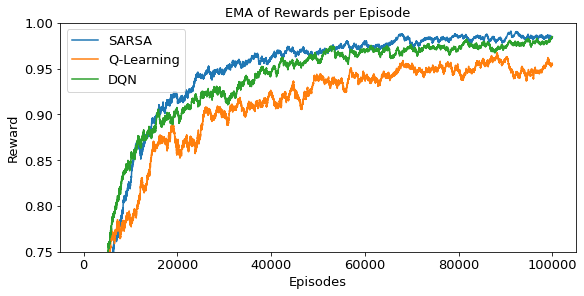
\includegraphics[width=.45\textwidth]{../figures/ema_rewards_per_episode_comparison.png}
    \caption{Exponential moving average of the rewards achieved during training. All three algorithms, Q-Learning, SARSA and DQN were initialized with identical weights and trained with identical network architecture and hyperparameters.}
    \label{fig:rewards}
\end{figure}

\begin{figure}
    \centering
    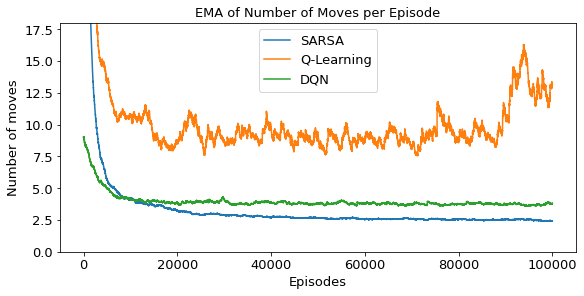
\includegraphics[width=.45\textwidth]{../figures/ema_number_of_moves_per_episode_comparison.png}
    \caption{\textcolor{red}{caption}}
    \label{fig:n_moves}
\end{figure}


We can see that, as expected, the rewards for Q-Learning are generally lower than the rewards for SARSA (Figure~\ref{fig:rewards}), because these figures depict the online learning and this chess environment is similar to the ``Cliff Walking'' environment, in that getting a draw and winning are closely related \cite{sutton2018}. In Figures~\ref{fig:n_moves} and \ref{fig:rewards} we can see that Q-Learning experiences instable learning behavior as it starts performing worse at around episodes 350000 and 100000. Even though the number of steps is not explicitly punished, the agents still learn to reduce the number of steps over time, as they do not give rewards and their goal is to take actions that do.

\textcolor{blue}{(5) Implement another Deep RL algorithm (it could be SARSA if you chose before Q
Learning and vice versa). Compare the new results with your previous results.}

As suggested by Mnih et al. \cite{atari2013}\cite{dqn2015}, DQN\footnote{Answer to task 5 for comparing DQN to SARSA and Q-Learning.} was able to overcome the downsides of Q-Learning which lead to an online performance which is comparable to that of SARSA in terms of reward and number of moves.

Since the above mentioned results could potentially be heavily influenced by the seed we chose a-priori, we decided to repeat the exact same experiment for 30 runs in order to get an idea of the average performance of each of the methods. For all runs we chose identical hyperparameters and model architecture to the original experiment without setting any seeds. For computational reasons we did however limit the number of episodes to 40000, which we think gives us a good general picture over the online performance as most of the training progress takes place before that.

For the learning curves see Figures~\ref{fig:30runs_reward} and \ref{fig:30runs_n_moves} in the appendix. We can observe that DQN and SARSA show very comparable learning curves with DQN showing slightly faster convergence in the first 5000 episodes. SARSA showed the lowest variance in all runs and seems to be a very stable algorithm. Q-Learning on the other hand showed clear signs of divergence as for some runs the rewards consistently dropped while the number of moves consistently increased. This shows that the measures taken by Mnih et al. \cite{dqn2015} to combat the disadvantages of Q-Learning worked and increased the stability as well as the convergence speed.

We can conclude that the seeded runs in our initial experiment truthfully represent the average run and therefore some level of inference is justified.


\subsection{Hyperparameters}



\textcolor{blue}{(4) Change the discount factor $\gamma$ and the speed $\beta$ of the decaying trend of $\epsilon$ (for a definition of $\beta$ please see code). Analyse the results.}

plot beta and gamma against performance metrics (maybe 3d). Interpret results.

We analyzed the impact of two hyperparameters on the learning process in detail\footnote{Answer to task 4.}: The discount factor $\gamma$, and the speed of the decaying trend of $\epsilon$, $\beta$. To do so, we decided to run the same model with 49 different combinations of $\gamma$ and $\beta$, with all other hyperparameters fixed to the ones we used for the seeded run. Also we used the same seed for initialization of the neural network weights and model architecture for all these runs, but we only ran the training for 40 episodes for computational reasons. We decided to use SARSA for this experiment, because as we already established, SARSA showed the lowest variance between runs and therefore serves as the best option to compare the outcomes, as, for instance, divergence problems can be ignored.

\begin{figure}
    \centering
\end{figure}


\textcolor{blue}{(6) [Group Only] Change the state representation or the administration of reward. Interpret your results.}

\textcolor{blue}{(7) [Group Only] The values of the weights could explode during learning. This
issue is called exploding gradients. Explain one possible way to fix this issue and
implement it. For example, search and study RMSprop). Show in a plot how your
solution fixed this issue.}








\section{Conclusion}\label{sec:conclusion}






\textcolor{red}{get correct bib format and complete entries}

\bibliographystyle{./IEEEtran}
\bibliography{./IEEEabrv,./Bibliography}

% \begin{thebibliography}{00}
%     \bibitem{atari2013} V. Mnih, K. Kavukcuoglu, D. Silver, D. Wierstra, A. Graves, I. Antonoglou, M. Riedmiller , ``Playing Atari with Deep Reinforcement Learning.'', CoRR, vol
%     % TODO: following entry is wrong
%     \bibitem{dqn2015} V. Mnih, K. Kavukcuoglu, D. Silver, D. Wierstra, A. Graves, I. Antonoglou, M. Riedmiller , ``Playing Atari with Deep Reinforcement Learning.'', CoRR, vol
%     \bibitem{sutton2018} R. S. Sutton and A. G. Barto, Reinforcement Learning: An Introduction., The MIT Press, 2018.

%     % todo: remove red color
%     \color{red}
%     \bibitem{b1} G. Eason, B. Noble, and I. N. Sneddon, ``On certain integrals of Lipschitz-Hankel type involving products of Bessel functions,'' Phil. Trans. Roy. Soc. London, vol. A247, pp. 529--551, April 1955.
% \end{thebibliography}

% todo: remove red color
\color{red}
\vspace{12pt}
IEEE conference templates contain guidance text for composing and formatting conference papers. Please ensure that all template text is removed from your conference paper prior to submission to the conference. Failure to remove the template text from your paper may result in your paper not being published.





\section{Appendix}
% todo: remove red color
\textcolor{red}{put the appendix after the bibliography?}


\begin{figure}[htbp!]
    \centering
    \begin{subfigure}[]{.45\textwidth}
        \centering
        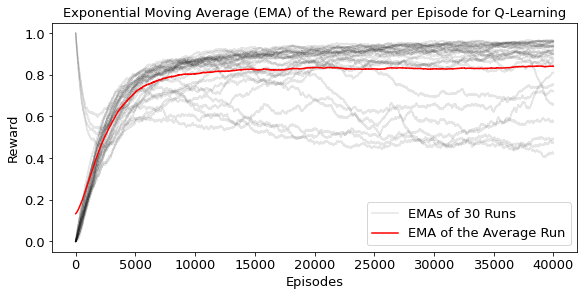
\includegraphics[width=\textwidth]{../figures/rewards_30_runs_qlearning.png}
        \caption{}
    \end{subfigure}
    \begin{subfigure}[]{.45\textwidth}
        \centering
        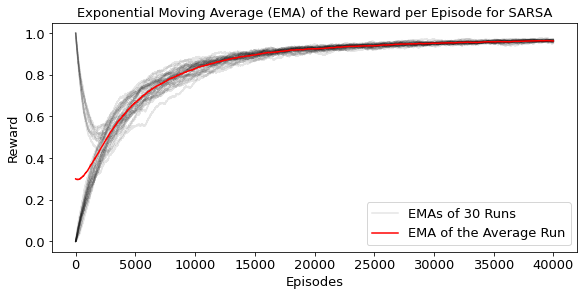
\includegraphics[width=\textwidth]{../figures/rewards_30_runs_sarsa.png}
        \caption{}
    \end{subfigure}
    \begin{subfigure}[]{.45\textwidth}
        \centering
        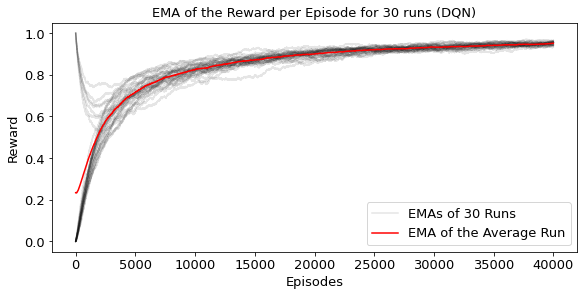
\includegraphics[width=\textwidth]{../figures/rewards_30_runs_dqn.png}
        \caption{}
    \end{subfigure}
    \caption{}
    \label{fig:30runs_reward}
\end{figure}
    

\begin{figure}[htbp!]
    \centering
    \begin{subfigure}[]{.45\textwidth}
        \centering
        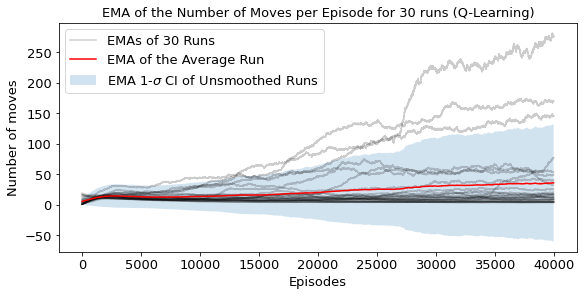
\includegraphics[width=\textwidth]{../figures/n_moves_30_runs_qlearning.png}
        \caption{}
    \end{subfigure}
    \begin{subfigure}[]{.45\textwidth}
        \centering
        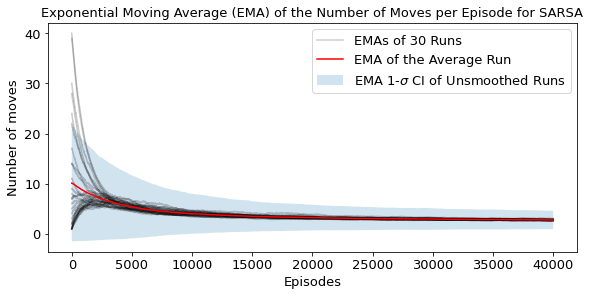
\includegraphics[width=\textwidth]{../figures/n_moves_30_runs_sarsa.png}
        \caption{}
    \end{subfigure}
    \begin{subfigure}[]{.45\textwidth}
        \centering
        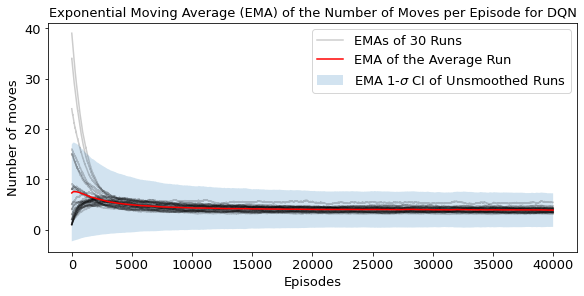
\includegraphics[width=\textwidth]{../figures/n_moves_30_runs_dqn.png}
        \caption{}
    \end{subfigure}
    \caption{}
    \label{fig:30runs_n_moves}
\end{figure}
    




\end{document}
